\documentclass{beamer}
\usetheme{Aalborg}

\usepackage{hyperref, graphicx, tgheros, minted, ulem}
\usepackage[utf8]{inputenc}
\usepackage[T1]{fontenc}

\title{Web Backend Development}
\subtitle{MSTC Technical Sharing}
\author{Richard Tsai}
\institute{Microsoft Student Technology Club,\\Sun Yat-sen University}
\date{\today}

\begin{document}
\begin{frame}[plain]
    \titlepage
\end{frame}

\begin{frame}{Agenda}
    \tableofcontents
\end{frame}

\section{Web App Basic Architechture}

\subsection{Frontend \& Backend}
\begin{frame}{Web App Basic Architechture}
    \center\Huge
    Frontend \& Backend
\end{frame}

\subsection{HTTP}
\begin{frame}{Web App Basic Architechture}
    \begin{block}{HTTP}
        \begin{itemize}
            \item What's HTTP? \pause
            \item B/S Architechture
                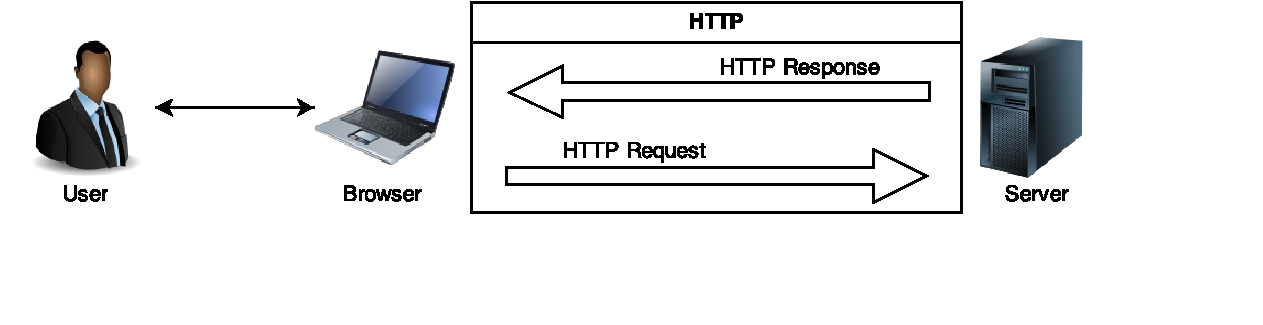
\includegraphics[scale=0.48]{http}
        \end{itemize}
    \end{block}
\end{frame}

\begin{frame}{Web App Basic Architechture}
    \begin{block}{HTTP Methods}
        \begin{itemize}
            \item GET
            \item POST
        \end{itemize}
    \end{block}
    \pause
    \begin{block}{``Stateless''}
        \begin{itemize}
            \item Cookies
            \item Session
        \end{itemize}
    \end{block}
\end{frame}

\begin{frame}[fragile]{Web App Basic Architechture}
    \begin{block}{HTTP Status Code}
        \begin{itemize}
            \item \verb|200 OK|
            \item \verb|301 Move Permanently| / \verb|302 Found| / \verb|303 See Other|
            \item \verb|404 Not Found|
            \item \verb|500 Internal Server Error|
        \end{itemize}
    \end{block}
\end{frame}

\section{Web Backend Development}

\subsection{Languages, Frameworks and etc.}
\begin{frame}{Web Backend Development}
    \begin{block}{Languages, Frameworks and etc.}
        \begin{description}
            \item[Python] Flask, Django, Bottle, \ldots
            \item[Ruby] Ruby on Rails
            \item[CLI Langs\footnotemark] ASP.NET MVC Framework
            \item[JavaScript] Node.js, Meteor, \ldots
            \item[PHP] Zend Framework, ThinkPHP, LazyPHP, \ldots
            \item[\sout{Java}] \sout{Spring, JFinal, Struts, \ldots}
        \end{description}
    \end{block}

    \footnotetext{C\#, VB.NET, C++/CLI, etc.}
\end{frame}

\subsection{A ``Hello world'' Example}
\begin{frame}{Web Backend Development}
    \center\Huge
    A ``Hello world'' Example
\end{frame}

\subsection{Database}
\begin{frame}[fragile]{Web Backend Development}
    \begin{block}{Database} \pause
        Structured Query Language (SQL)
        \begin{minted}[fontsize=\scriptsize]{sql}
INSERT INTO `tbl` (`name`, `grade`) VALUES ('wodesuck', 2012)
DELETE FROM `tbl` WHERE `name` = 'wodesuck'
SELECT `id`, `name`, `grade` FROM `tbl` WHERE `grade` = 2012
UPDATE `tbl` SET `grade` = 2013 WHERE `id` = 10
        \end{minted}
    \end{block}
\end{frame}

\subsection{Architechture Patterns}
\begin{frame}{Web Backend Development}
    \begin{block}{Architechture Patterns} \pause
        Model-View-Controller (MVC)

        \center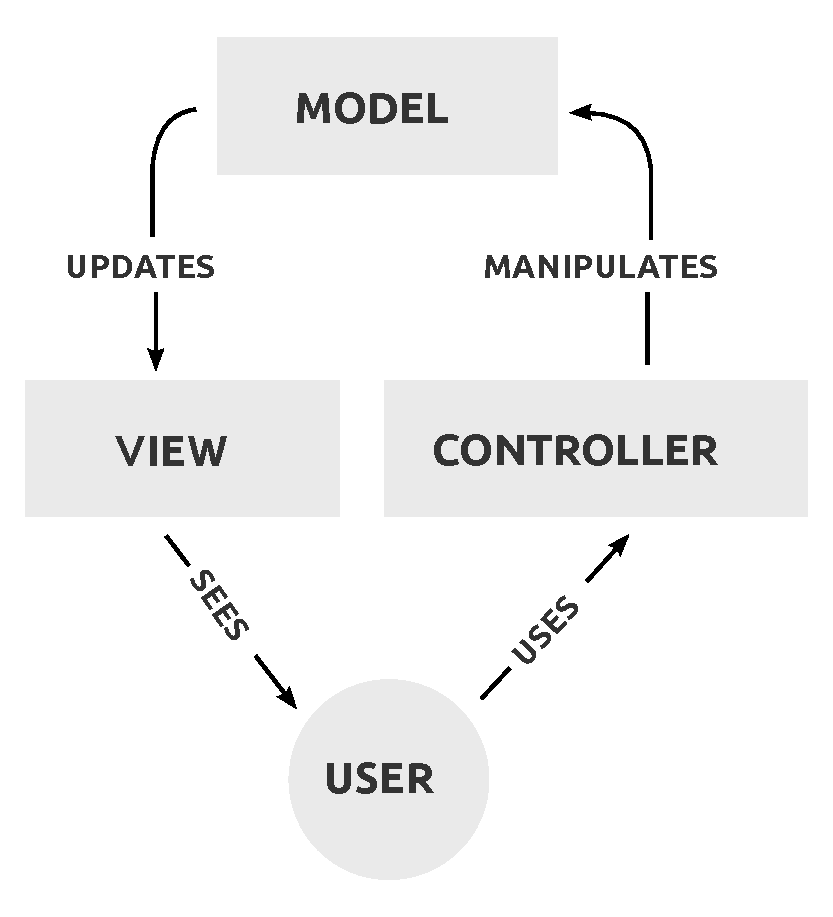
\includegraphics[scale=0.36]{MVC}\footnotemark
    \end{block}

    \footnotetext{Image from Wikipedia}
\end{frame}

\subsection{Security}
\begin{frame}{Web Backend Development}
    \begin{block}{Security} \pause
        \begin{itemize}
            \item SQL Injection
            \item XSS
            \item CSRF
            \item etc.
        \end{itemize}
    \end{block}
\end{frame}

\section{Completed Architechture}

\subsection{Case Study: MSTCWEB}
\begin{frame}{Completed Architechture}
    \begin{block}{Case Study: MSTCWEB} \pause
        \center
        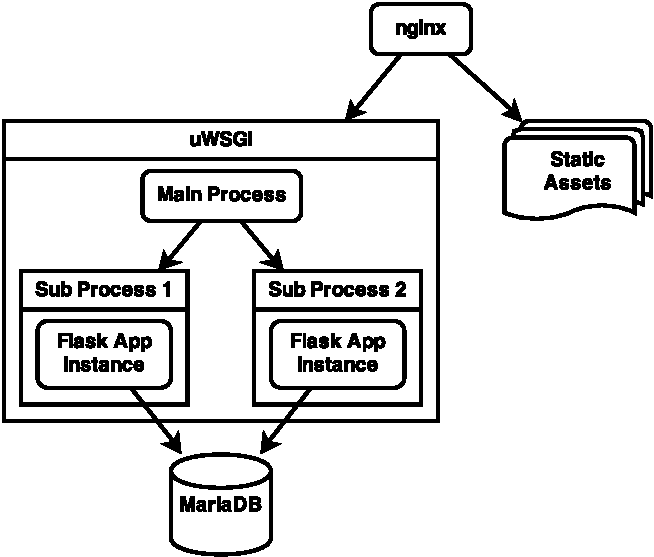
\includegraphics[scale=0.6]{mstcweb}
    \end{block}
\end{frame}

\section{Others}

\begin{frame}{Others}
    \begin{block}{Tools}
        \begin{itemize}
            \item Chrome Developer Tools
            \item phpMyAdmin
        \end{itemize}
    \end{block}
    \pause
    \begin{block}{Deployment Platform}
        \begin{itemize}
            \item Physical Server, VPS and IaaS
            \item PaaS
        \end{itemize}
    \end{block}
\end{frame}

\subsection{Resources}

\begin{frame}{Others}
    \begin{block}{Resources}
        \begin{description}
            \item[W3School\bf s] \href{http://w3schools.com}{\tt http://w3school{\bf s}.com}
            \item[W3School] \url{http://w3school.com.cn}
            \item[MDN] \url{https://developer.mozilla.org}
        \end{description}
    \end{block}
\end{frame}

\end{document}
